%\documentclass[11pt,a4paper]{scrartcl}
\documentclass[12pt]{article}

\usepackage[top=2.0cm, right=2.0cm, left=2.0cm, bottom=2.0cm]{geometry}

%\usepackage{setspace}
%\doublespacing

%\usepackage[left]{lineno}
%\linenumbers

\usepackage[utf8]{inputenc}
\usepackage[UKenglish]{babel}
%tableau
\usepackage{array, multirow}
%graphs
\usepackage{multicol}
\usepackage{url}
\usepackage{graphicx}
\usepackage{float, caption}
\usepackage{amsmath,amssymb,mathrsfs}
\usepackage{natbib}

\usepackage{graphicx}
\usepackage{color}
\usepackage{pgf}
\usepackage{tikz}
\usetikzlibrary{arrows,snakes,backgrounds}

%pour avoir la biblio avec nom d'auteur et année dans le texte
\bibpunct{(}{)}{;}{a}{,}{,}
%pour avoir les reference entre parenthese et en cas de ref multiple séparé par des ;
\sloppy 
%utiliser ca si latex trop exigeant en largeur ligne

\title{Chaotic but regular recurrent influenza epidemics: from theory
  to observation}

%other title proposals
%\title{Chaotic dynamics with uniform phase in influenza
%  epidemics: from theory to observation}

\author{Sébastien Ballesteros$^{1,*}$, Lewi
  Stone$^{2}$,  Anton Camacho$^{1}$\\ Elisabeta Vergu$^{3}$, Bernard Cazelles$^{1,4}$}

\date{}

\begin{document}

\maketitle


$^1$UMR 7625  (UPMC, ENS, AgroParisTech, CNRS), Ecole Normale
Supérieure, Unit of Eco-Evolutionary Mathematics,  46 rue d'Ulm,
F-75230 Paris Cedex 05, France. \\
$^2$Biomathematics Unit, Faculty of Life Sciences, Tel Aviv
University, Ramat Aviv 69978, Israel \\
$^3$~INRA, UR341 Mathématiques et Informatique Appliquées, F-78352 Jouy en Josas, France \\
$^4$~IRD UR GEODES, 93142 Bondy, France

~\\
$^*$\textit{Corresponding author}:  \\
E-mail: sebastien.ballesteros@biologie.ens.fr

\section*{Abstract}


Human Influenza epidemics in temperate areas are characterised by
a relatively constant phase (despite influenza type or subtype
alternates) and highly variable amplitude. Influenza epidemics peaks
variability is currently explained by punctuated evolution of
influenza main antigen, higher peaks reflecting higher antigenic
changes.  We seek to determine to what extent gradual antigenic drift
alone (without perturbations of rare mutations with strong antigenic
effects) and therefore non-linear dynamics by itself can induce
Uniform Phase and Chaotic Amplitude (UPCA) dynamics. We present a
minimal model taking into account key processes of influenza
epidemiology and evolution. We show that this model present UPCA
dynamics for a wide range of parameter value relevant for influenza
A. We then confirm the presence UPCA dynamics in real data and show
the robustness of UPCA dynamics on a worldwide metapopulation model
including age structure and realistic infectious time
distribution. Finally, we argue that chaotic dynamics with uniform
phase should be the baseline scenario to consider when trying to
interpreter influenza epidemics size variability.  Influenza UPCA
dynamics therefore sets fundamental limits to the predictability of
future epidemics sizes in addition to evolutionary contingency.

~ \\
\textit{Keywords}: \\
Influenza, Gradual Antigenic Drift, Chaos, UPCA Dynamics, State-Space
Model, Particle Filter.

\section{Introduction}
\label{sec:introduction}

Interpandemic human influenza appears annually in most temperate
climatic zones of the world with epidemics that peak in the cold
winter months. These outbreaks have been documented in the scientific
literature in records that extend back to at least 1650
\citep{Potter2001}, making it an exceptional example of a persisting
recurrent disease.  Being a respiratory infection, and highly
infective at that, influenza spreads from person to person in the form
of virus aerosol particles, and has the ability to propagate rapidly
through human populations. Average epidemics may have attack rates of
the order of 10-20 \% in cities but in certain susceptible populations
(school-children, nursing homes) the levels may reach 40-50 \%
\citep{Cox2000a}.  Influenza is thus a source of considerable human
morbidity and mortality, reaching some 250,000 to 500,000 deaths per
year globally, and clearly exacting a large overall economic toll on
society.

There is still much controversy in identifying the seasonal drivers
that generate annual influenza oscillations, and the processes that
give rise to their large variability \citep{Finkelman2007}. These are
in fact outstanding problems of influenza research today, and are
addressed in detail from a modeling perspective here. As is well known
from the many studies of childhood infectious diseases, a necessary
requirement for the generation of recurrent epidemics is a sufficient
and continuous source of new susceptible individuals arising in the
population; enough to fuel each new outbreak. In the classical 1977
experiments of \citet{Potter1977} and \citet{Gill1977}, it was
established that although hosts infected with influenza gain immunity,
ultimately they may become susceptible once again and reinfected due
to the rapidly evolving nature of the influenza virus.  Positive
selection exerted by the host immune system, leads to a continual
antigenic drift of the influenza virus's glycoproteins, particularly
the main antigen hemagglutinin (HA), thus allowing the virus to
eventually evade the immune system.  The process of antigenic drift
thereby creates an important renewed source of susceptible
individuals.  Evolutionary forces are thus considered to be of
tremendous importance in shaping complex recurrent patterns of
infectious diseases \citep{Cobey2008}, and are the reasons why
influenza is widely regarded as an invariable disease caused by a
variable virus \citep{Potter2001}.

Recently, new theoretical developments along with recent data,
analyzed by phylogenetic and coalescent based approaches
\citep{Smith2004, Koelle2006, Wolf2006, Rambaut2008} have revealed
that the evolution of influenza A H3N2 main antigen (HA) is punctuated
with discrete antigenic clusters jumps. Epochal evolution,
materialised by sudden change of pathogens either due to mutations or
re-assortments can have large epidemiological impacts. Punctuated
immune escape therefore offers an intuitive explanation to the time
series of Human Influenza epidemics in temperate areas. Within the
scope of epochal evolution higher peaks can reflect higher antigenic
changes \citep{Koelle2006}.

The recent emphasis on punctuated immune escape has been the source of
important discussions with some authors rejecting epochal evolution in
favour of a more gradual immune escape pattern \citet{Shih2007,
  Suzuki2008}. In this papers we add new arguments to the debate by
focusing on the information that can be inferred from influenza
incidence time series at the population level.  We seek to contrast
``an extrinsic view'' \citep{Cobey2008} of influenza dynamics where
antigenic cluster transitions induce epidemic amplitude variability
and higher peaks reflect larger antigenic changes, with ``an intrinsic
view'' of purely gradual evolution where epidemic size variability can
only result from the internal nonlinear dynamics of the system.

Our modeling effort focuses on the dynamics of influenza A, given that
of the different influenza types, A contributes most to human disease
burden.  We begin by formulating a minimal mathematical model that
characterizes its dynamics as having Uniform Phase, or regular
periodicity in rhythm, together with epidemic peaks having irregular
Chaotic Amplitudes; a phenomenon referred to here in short as UPCA.
We confront our modeling results with time series data and argue that
UPCA dynamics should be the baseline scenario to consider when trying
to interpret the complex population dynamics of recurrent influenza
epidemics.  As seen in Figure~\ref{fig:attractor}, long-term influenza
timeseries from both France and Israel (Figure S1) make evident that
the UPCA dynamics are an obvious feature.  To our knowledge, no
previous deterministic modeling attempts of single or multi-strain
dynamics have been able to reproduce the fundamental characteristics
of UPCA which are inherent in many observed influenza timeseries.
These findings around the nonlinear nature of the mechanisms of
transmission highlight that in addition to evolutionary contingency
diseases like influenza have fundamental limits to the predictability
of future epidemics sizes.




\begin{figure}[htb]
  \center
  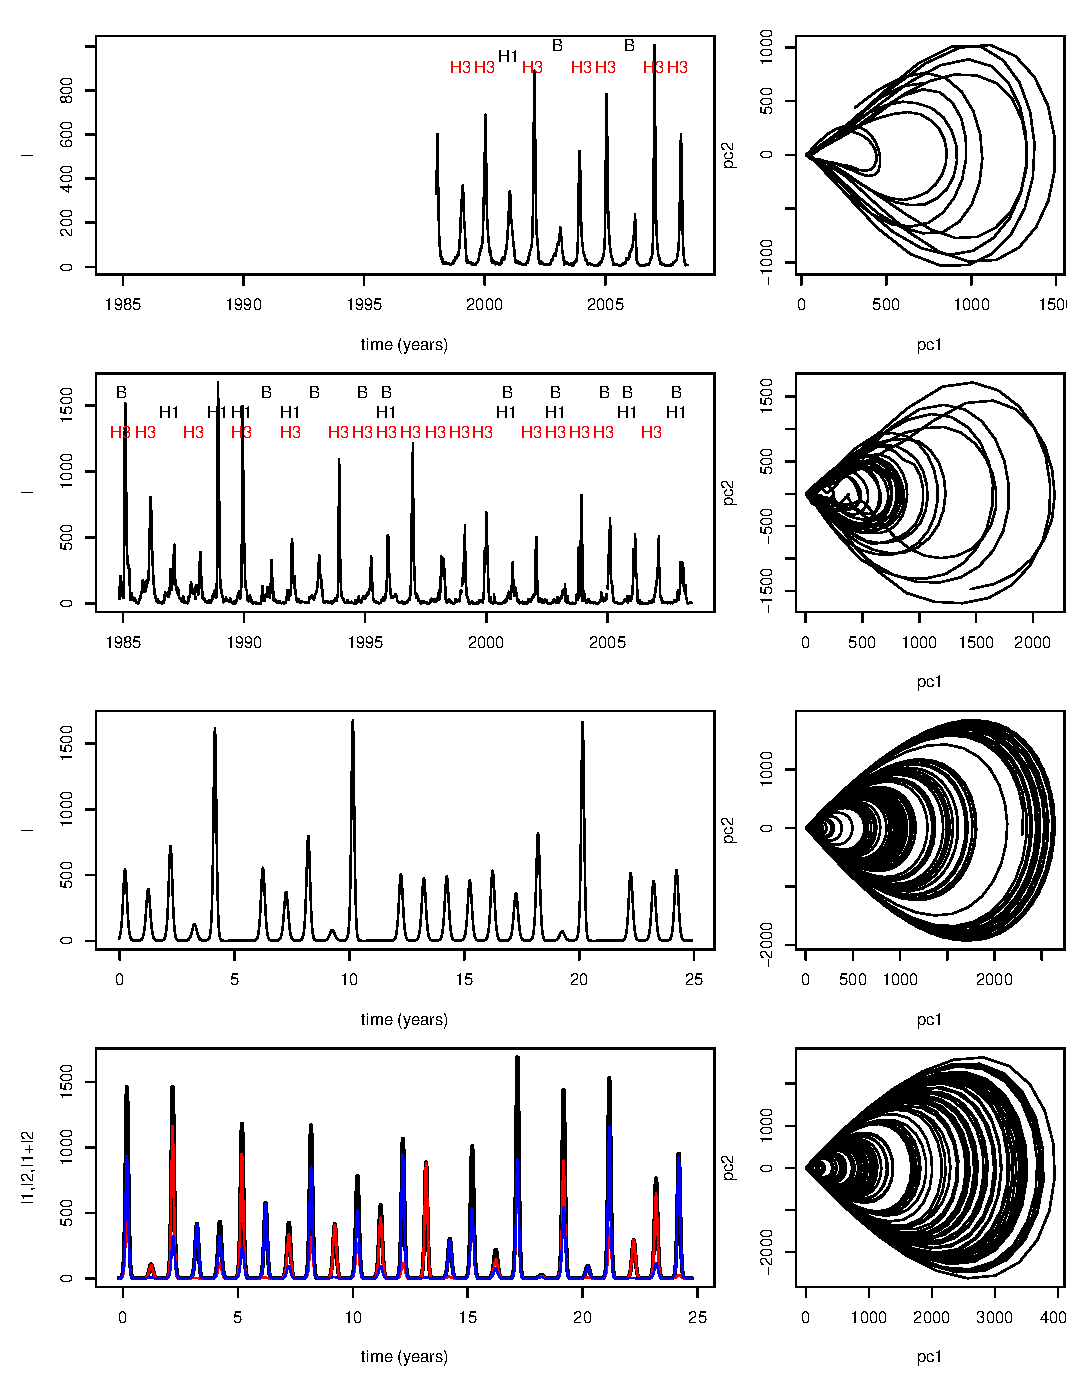
\includegraphics[width= 0.8 \linewidth]{graph/all_reconstructed_bernard.eps}
  \caption{Weekly incidence rates for Influenza Like Illness
    per 100 000 hosts in Ile de France and Israel:
    First line: Data from for region Ile de France. 
    Second line: Data from Israel.
    Other lines: Typical weekly incidence rate output for the
    determinist single subtype $SIRS$ model (first line) and the
    determinist 2 subtype model (third line).
    % 
    Right graphs are phase state representation (after a principal
    component analysis)  with embedding realised by the method of delay.
    % 
    Parameters: third line maximum likelihood estimate for Paris
    ($R_0=1.65$, $1/\nu=2.47$ days$^{-1}$, $1/g=7$ years$^{-1}$,
    $e=0.104$, $\eta=10^{-6.7}$) ; fourth lines: empirical parameter
    set with $e=0.2$, $1/g=25$ years$^{-1}$, $1/q=6$ months$^{-1}$,
    $1/ \gamma=1.5$ days$^{-1}$.}
  \label{fig:attractor}
\end{figure}


\section{Theory}
\label{sec:theory}

\subsection{A minimal model for influenza A}
\label{sec:model}


We consider a minimal model that takes into account three key
processes of influenza dynamics in temperate areas: seasonal forcing,
external reintroductions and antigenic drift \citep{Nelson2007}.

The importance of the role of seasonal forcing has long been
acknowledged and is best observed by comparing influenza seasonal
patterns along a latitude gradient: the seasonal patterns range from
marked seasonal winter activity centred around January in the Northern
hemisphere, to uniform circulation throughout the year in the Tropics
and again, strong winter epidemics center around July in the Southern
hemisphere \citep{Viboud2006}. Climatic triggers appear to be involved
\citep{Alonso2007a} and influenza transmission has been reported to be
controlled by temperature and relative humidity \citep{Lowen2007}.
However, a precise understanding of what drives seasonal influenza
trends has not yet been achieved \citep{Finkelman2007, Lofgren2007}. A
further complication may be linked to the fact that although
seasonality may appear to dominate, its intensity might not
necessarily be strong if there is dynamical resonance as speculated in
\citep{Dushoff2004}.

Related to the seasonal patterns of influenza, recent developments
made possible through the availability of large genetic data sets,
have revealed that global influenza is a source-sink system, with the
tropics constantly reseeding the temperate areas \citep{Rambaut2008,
  Russell2008}. The antigenic change observed in temperate populations
seems to be a secondary effect of strong selection within, and largely
unidirectional flow from the source population where sustainable year
long transmissibility favour successful antigenic changes. This
advance renders migration and influenza re-introduction key processes
to consider when one studies the dynamics of influenza across seasons
in temperate areas.

As already stated, the punctuated versus gradual nature of antigenic
drift is currently highly debated. Previous studies have derived
estimates of the rate of antigenic drift. Data from \citet{Potter1977}
revealed that the probability of reinfection increases linearly with
time since last infection due to an average antigenic drift rate
estimated to be 1/19.5 years$^{-1}$ \citep{Pease1987}. Statistical
inference methods as used in \citet{Finkenstaedt2005}, have resulted
in estimates of 1/13 years$^{-1}$ with a model accounting only for
purely gradual antigenic drift and estimates of 1/23.3 years$^{-1}$
for the gradual component in a model that allows for punctuated
evolution and discrete antigenic change (see also \citet{Xia2005} for
a semiparametric approach).


Taking into account these three key processes results in the model of
equation~\eqref{eq:sirs} that is described in figure~\ref{fig:sirs}
and presented in the Method.


\begin{figure}[htb]
  \center
  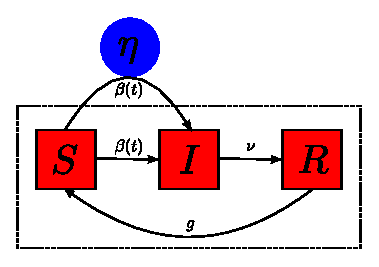
\includegraphics[width= 0.3 \linewidth]{graph/sirs.eps}
  \caption{A minimal model for a given subtype of influenza A: $S$ is
    the number of susceptible hosts, $I$ the number of infectious
    hosts and $R$ the number of recovered and temporary immunised
    hosts. $\beta(t)$ is the transmission rate taking into account
    seasonality, $\nu$ the recovery rate, $g$ the antigenic drift rate
    (due to viral evolution) and $\eta$ is the contribution of
    infectious hosts from external regions to the force of infection.}
  \label{fig:sirs}
\end{figure}

In order to study the dynamics of the models of eq~\eqref{eq:sirs}
and~\eqref{eq:HB}, we make use of two sets of parameters. One consists
of parameters commonly adopted in theoretical papers (\textit{e.g.}
\citet{Koelle2006, Ferguson2003, Goekaydin2007}) and the other
consists of more direct estimates of parameters from household studies
(\textit{e.g.} \citet{Cauchemez2004, Lavenu2004, Ferguson2005}). Both
parameter sets are listed in Table~\ref{tab:param}.  The remaining
parameters ($e$ $g$ and $\eta$) are considered as bifurcation
parameters.

\begin{table}[htb]
  \center
  \begin{tabular}{|l|l|l|}
    \hline
    Parameters & Theoretical & Empirical\\
    \hline
    $\nu$ (recovery rate) & $1/8$ days$^{-1}$ \citep{Koelle2006} & $1/2.77$ days$^{-1}$ \citep{Lavenu2004} \\
    \hline	
    $R_0$ ($\beta=R_0 \nu$) & $5$ \citep{Koelle2006} & $2.66$ \citep{Lavenu2004} \\
    \hline		
  \end{tabular}
  \caption{Parameter values}
  \label{tab:param}
\end{table}

The first model with one sub-type can be easily generalized for
co-circulating subtypes assuming that subtypes only interact via a
temporary period of full cross-immunity as suggested by
\citet{Webster1992}. A such model has also be analyzed with
two-subtypes (see Methods and figure~\ref{fig:2subtypes}),
representing for instance the co-circulation of H3N2 and H1N1
influenza A subtypes as has been the case since 1977 \citep{Earn2002}.

\begin{figure}[htb]
  \center
  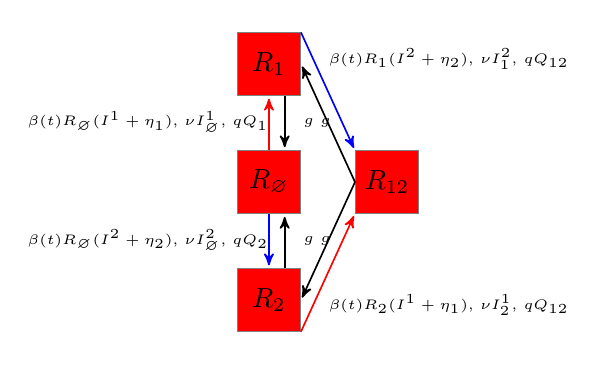
\begin{tikzpicture}[node distance=1.5cm, inner sep=0pt, minimum size=8mm]
    
    \tikzstyle{seb}=[rectangle, fill=red, draw=gray, text=black] \tikzstyle{I1}=[->,   draw=red, shorten >=1pt, >=stealth',semithick]                     \tikzstyle{I2}=[->,draw=blue, shorten >=1pt, >=stealth',semithick] \tikzstyle{g1}=[->,shorten >=1pt, >=stealth',semithick]                     \tikzstyle{g2}=[->,shorten >=1pt, >=stealth',semithick]
    
    \node[seb] (R0) {$R_\varnothing$}; \node[seb] (R1) [above of=R0] {$R_1$}; \node[seb] (R2) [below of=R0] {$R_2$}; \node[seb] (R12) [right                    of=R0] {$R_{12}$};
    
    \draw[I1] (R0) to node[auto] {\begin{tiny}$\beta(t) R_\varnothing
        (I^1 +\eta_1)$, $\nu     I_\varnothing^1$, $qQ_1$\end{tiny}} (R1) ;
    \draw[I2] (R0) to node[auto,swap] {\begin{tiny}$\beta(t)
        R_\varnothing  (I^2 +\eta_2)$, $\nu     I_\varnothing^2$, $qQ_2$\end{tiny}} (R2);
    \draw[I2] ([yshift=+4mm] R1.east) to node[auto]
    {\begin{tiny}$\beta(t) R_1 (I^2 +\eta_2)$, $\nu     I_1^2$, $qQ_{12}$\end{tiny}} ([yshift=+4mm] R12.west) ;
    \draw[I1] ([yshift=-4mm] R2.east) to node[auto,swap]
    {\begin{tiny}$\beta(t) R_2 (I^1 +\eta_1)$,     $\nu I_2^1$, $qQ_{12}$\end{tiny}} ([yshift=-4mm] R12.west) ;
    \draw[g1] ([xshift=+2mm] R1.south) to node[auto] {\begin{tiny}$g$ $g$\end{tiny}} ([xshift=+2mm] R0.north) ;
    \draw[g2] ([xshift=+2mm] R2.north) to node[auto,swap] {\begin{tiny}$g$ $g$\end{tiny}} ([xshift=+2mm] R0.south) ;
    \draw[g1] (R12.west) to (R2.east) ;
    \draw[g2] (R12.west) to (R1.east) ;
  \end{tikzpicture}
  \caption{A minimal model for two subtypes of influenza A interacting
    via a short period of full cross-immunity ($Q$) of average
    duration $1/q$. With the notation of eq~\eqref{eq:HB}
    $J=\{\{\varnothing\}, \{1\}, \{2\}, \{1,2\}\}$ and trace the
    current level of immunity; $k=1, 2$ and indexes the co-circulating
    subtypes.  Infection (transition from states $R_J\setminus k$ to
    $R_J$) are represented by red and blue arrows for subtypes 1 and
    2. During the transition hosts pass through states $I^k_J\setminus
    k$ and $Q_J$ as denoted on the arrows.  As the viral population
    evolves, hosts can loose immunity (black arrows).}
  \label{fig:2subtypes}
\end{figure}

\subsection{UPCA dynamics in influenza epidemics}
\label{sec:res_upca}

As mentioned above, UPCA dynamics is a good candidate to explain
influenza incidence time series in the absence of rare mutation and
with strong antigenic effects. The uniform phase characterizes the
regular annual outbreak, while the chaotic amplitudes of the number of
infectives characterizes the irregular amplitude of the epidemics from
year to year.  We will shortly show that the simple models outlined
above naturally generate UPCA dynamics.

To our knowledge UPCA dynamics was first introduced in theoretical
biology by \citet{Blasius1999} in the context of the tritrophic
vertical Canadian Lynx-hare-vegetation foodweb.  Contrary to
ecological foodweb models \citep{Stone2007}, for epidemiological
systems represented by the classical forced $SIR$ model we have found
that it is difficult, if not impossible, to locate parameter regimes
in which outbreaks occur regularly each year. For $SIR$ systems, there
are a significant number of years in which major epidemics do not
appear to trigger at all, i.e., they ``skip'' \citep{Stone2007a,
  Olinky2008}., and this is an intrinsic feature of these models.

In contrast, the $SIRS$ models with immigration (eq.~\eqref{eq:sirs}
and~\eqref{eq:HB}) proves to be good candidates for UPCA dynamics
because of the higher rate of susceptible renewal provided by
antigenic drift and by the presence of external infections, both of
which precipitate epidemic ``re-birth'' after large events of
susceptible depletion.  Figure~\ref{fig:attractor}, Sx and Sxx display
typical model realizations of Eqns.~\eqref{eq:sirs} and~\eqref{eq:HB}
and makes clear the strong annual outbreak, although the intensity of
the outbreak is quite different, and in fact chaotic, from year to
year.

It was important to assess whether UPCA dynamics is a commonplace or a
pathological feature by scanning the dynamics over a large range of
parameter space. That UPCA dynamics is chaotic, means that it can be
detected by checking for a positive first Lyapunov exponent following
the algorithm of \citep{Wolf1985}).
Phase regularity was identified by demanding than 95\% of the
inter-peak intervals ranged between 0.7 and 1.3 years (others measures
for phase stability do not significantly alter the results). To ensure
that we do not select trajectories containing ``skips'', we retained
only time series having all maxima with amplitudes that are higher
than 5\% of the endemic equilibrium in the absence of seasonal
forcing. This value was found appropriate to allow years with very low
peak (akin to refractory period reported by Koelle et al. (2006) after
antigenic cluster transitions) but sufficiently high to ensure that
the following year was marked with a significant peak (in accord with
data).

Figure~\ref{fig:main2} and~\ref{fig:eta_best_fit2} reveals the results
of the bifurcation analysis for both the one subtype and two subtype
models. In all cases, UPCA dynamics occurs in wide areas of realistic
parameters values for influenza. In particular, UPCA dynamics are
possible for antigenic drift values compatible with estimates of
\citet{Finkenstaedt2005} and \citep{Pease1987} who report gradual
antigenic drift rates ranging from 1/13 to 1/25 years$^{-1}$.

As can be seen in figure~\ref{fig:attractor}, Sx and Sxx it is
striking how the single subtype SIRS UPCA model is able to produces
patterns reminiscent of antigenic cluster transition, (years with a
significantly higher peak followed by a refractory period of one year)
with only purely gradual antigenic drift. Even more surprising, the
period in between those refractory period correspond closely to the
reported duration of antigenic cluster persistence ranging for 1 to 8
years \citep{Smith2004}.


\begin{figure}[htb]
  \center
  \includegraphics[width= 0.8 \linewidth]{graph/main2.eps}
  \caption{First lyapunov exponent and parameters space where we
    expect UPCA dynamics (black contours). Top : single subtype model
    ; bottom : Two co-circulating subtypes model for an average 6
    months period of temporary full cross-immunity.  Parameters: Left:
    $R_0=5$ ; $1/\nu=8$ days ; $\eta=1.10^{-6}$ corresponding to
    \citep{Koelle2006}. Right: $R_0=2.66$ ; $1/\nu=2.77$ days ;
    $\eta=1.10^{-7}$ corresponding to
    \citep{Lavenu2004}. Supplementary figure in the appendix details
    the periods bifurcations.}
  \label{fig:main2}
\end{figure}


\section{Corroborations from observations}
\label{sec:confirmation}

First we simply compare qualitatively the time series and the
attractors of the observation and simulation of the models. Figure
\ref{fig:attractor} presents a phase space representation of the ILI
data from Ile de France and Israel as well as comparisons with two
dimensional projections of the strange attractors of the model of
eq~\eqref{eq:sirs} and~\eqref{eq:HB} (two subtype case). All these
graphs show general good agreement between the theoretical and the
reconstructed phase space representation.

To confirm these qualitative results, we have compare the UPCA model
to real data, by implementing a stochastic version of
eq~\eqref{eq:sirs} (see Electronic Supplementary Materials) and using
maximun likelihood identification. Parameter inference was achieved
with an implementation of maximum likelihood via iterated filtering
(MIF) as described in \citet{Ionides2006} and \citet{Breto2009} (see
Electronic Supplementary Materials).


The results of the inference procedure are depicted in figure S. The
transmission and antigenic drift rates were difficult to estimate and
appeared to be strongly correlated as can be seen in figure S. This
correlation is a cause of concern for studies estimating the basic
reproductive number of influenza based on the first growing parts of
the epidemic curve and therefore neglecting the effect of antigenic
drift (\textit{e.g.} \citet{Chowell2008a}). If such studies provide
valuable insights to the value of $R$, the link to $R_0$ is difficult
to made \citep{McVernon2007, Mathews2009} and we found that a given
level of infective with the same overall qualitative dynamics could be
achieved by modifying either $\beta_0$ or $g$.

We then examine to what extent the parameters inferred in figure S
were compatible with UPCA dynamics. Due to the uncertainty of the
antigenic drift rate and given the difficulty to directly insert the
external infection parameter from the stochastic model to the
deterministic model (eq~\eqref{eq:sirs}) we considered $g$ and $\nu$
as bifurcation parameters and fixed the other parameters to their
maximum likelihood value.

Figure \ref{fig:eta_best_fit2} reveals that these parameter inferred
for ILI data of region Ile de France are within the UPCA area of the
deterministic model for a large range of $g$ and $\nu$ values. All
these results corroborate the interest of the UPCA dynamics in
influenza epidemics.
% Moreover it is important to specify that the simulated time series
% presented Fig. 1 and Fig. S have been obtained with the parameter
% inferred from ILI data of region Ile de France.



% As most of the estimate for $R_O$ are between 1.5 and 2
% \citep{Lessler2007} we fixed $R_0$ to its best estimates of 1.65.

\begin{figure}[htb]
  \center
  \includegraphics[width= 0.8 \linewidth]{graph/eta_best_fit2_g11.eps}
  \caption{One dimensional and two dimensional bifurcation diagram for
    external infectious hosts parameter ($\eta$) and antigenic drift
    rate ($g$) . Other parameters are fixed at their maximum
    likelihood estimate from figure~S ($R_0=1.65$,
    $1/\nu=2.47$ days$^{-1}$, $e=0.104$,
    $\eta=10^{-6.7}$). Supplementary figure in the appendix details
    periods bifurcations.}
  \label{fig:eta_best_fit2}
\end{figure}

\section{Robustness}
\label{sec:robustness}

Due to the growing recognition of the punctuated nature of immune
escape \citep{Cobey2008} we have checked to what extent UPCA dynamics
are robust to rare mutation with higher than usual antigenic
effects. For this purpose, we have generalised the model of
eq.~\eqref{eq:sirs} so that at random times, a percentage $x \in
[0,1]$ of recovered hosts became susceptible again. In order to
quantify the magnitude of $x$ we have used the ratio of the maximum
number of infected host in the presence of perturbations over the
maximum number of infected host for a typical unperturbed UPCA
trajectory. This ratio is plotted in figure~\ref{fig:pert} (right
panel).  Contrasting this ratio to the ILI data, enabled us to set a
maximum boundary $x<0.07$ . This value is in accord with
\citep{Finkenstaedt2005} study who estimated $x$ values for french ILI
data all smaller than 7\% with 53\% of the estimates $\leq 2\%$ ;
26.7\% between 2 and 5 \% and 20\% between 5 and 7 \%.
Figure~\ref{fig:pert} reveal that UPCA dynamics is robust to such
perturbations, the transient being shorts.  As suggested by
\citep{Koelle2006}, we also notice that punctuated immune escape can
induce higher peaks followed by refractory periods. However the
occurrence of such a pattern strongly depends on the time of the
perturbation and is not systematic.

\begin{figure}[htp]
  \center
    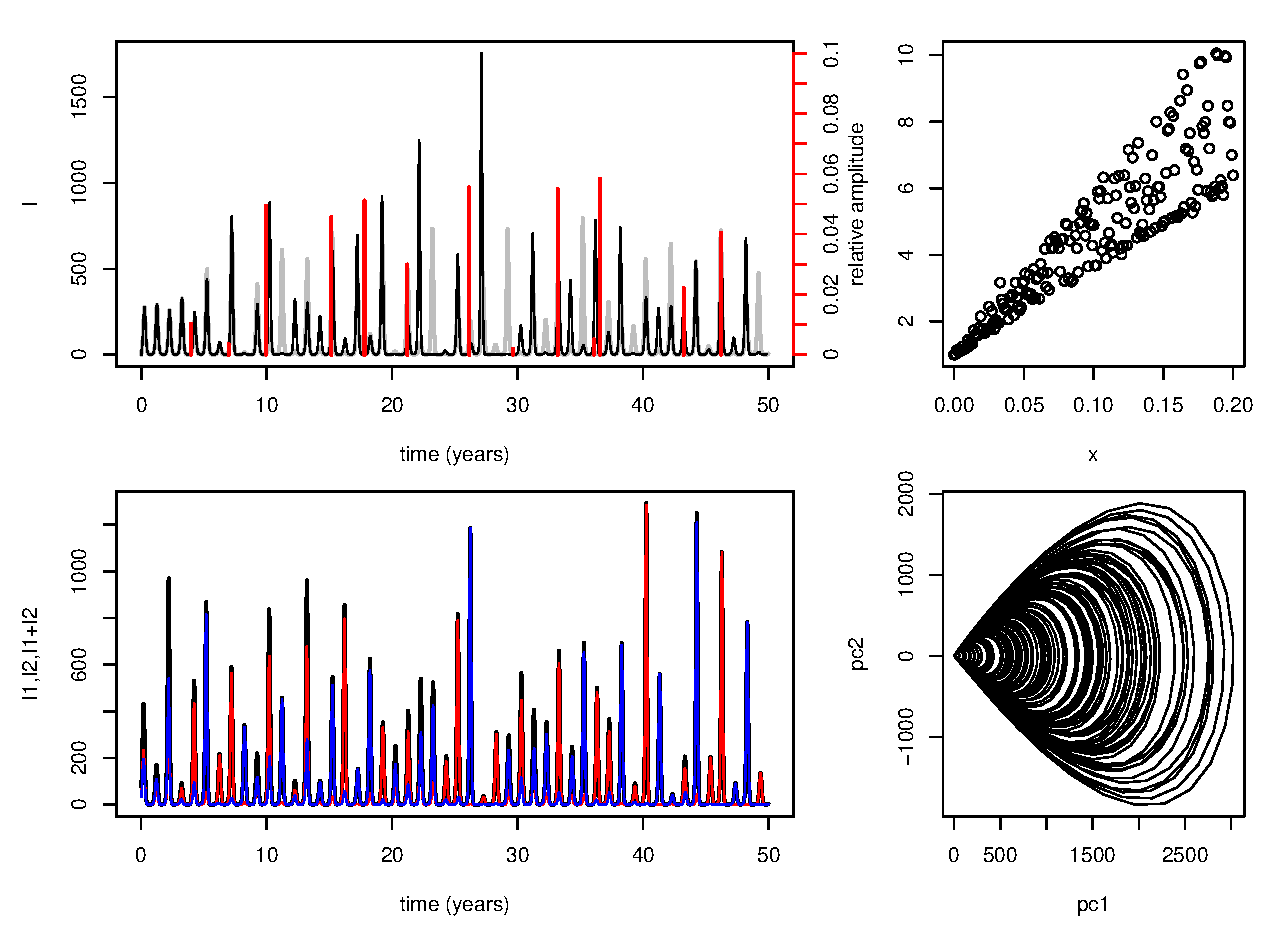
\includegraphics[width= 0.8 \linewidth]{graph/pert.eps}
    \caption{Robustness of UPCA dynamcis.
      % 
      First line: effect of environmental stochasticity. Left panel:
      Gray line a UPCA unperturbed trajectory (parameters:
      ($R_0=1.65$, $1/\nu=2.47$ days$^{-1}$, $1/g=11$ years$^{-1}$,
      $e=0.104$, $\eta=10^{-6.7}$) Black line: perturbed trajectory,
      red lines indicate times when $x$ percent of $R \to
      S$. Perturbation times are sampled from a gaussian distribution
      with mean=3.3 and sd=1.9 corresponding to value of antigenic
      cluster succession reported by \citep{Smith2004}. Perturbation
      intensity are sampled from a uniform law of parameter 0,0.07 as
      determined by right panel described in the main text.
      % 
      Second line: A typical realization of the stochastic
      metapopulation model for Paris and the associated phase state
      representation (after a principal component analysis) with
      embedding realised by the method of delay obtained with the
      empirical parameter set. Other parameter are $1/g=25$
      years$^{-1}$, $1/q=6$ months$^{-1}$, $1/ \gamma=1.5$
      days$^{-1}$). Seasonal forcing ($e=0.2$) for Northern and
      Southern hemisphere cities are in phase opposition and tropics
      do not present seasonality.}
  \label{fig:pert}
\end{figure}

The robustness of the UPCA dynamics was then tested by increasing the
realism of the model in various ways.  First, we constructed a
stochastic metapopulation version of the model of eq~\eqref{eq:HB}
with realistic inter-city migration routing as based on transportation
data flow from 52 cities published in \citep{Grais2003} (see
Electronic Supplementary Materials). Second, more realistic infection
time distributions were employed by incorporating an exposed class
($E$) and by using Erlang infectivity distributions instead of
exponential. Third, the population was modeled with three age classes
using \citet{Wallinga2006} data from social contacts to estimate
age-specific transmission parameters. The full model is written in
methods eq~\eqref{eq:full}.  Figure~\ref{fig:pert} and S reveals the
robustness of UPCA dynamics that appears little affected by
demographic stochasticity, metapopulation dynamics, age structure and
non exponential infected time distribution.


\section{Discussion}
\label{sec:discussion}

%1-
The studies of \citet{Smith2004, Koelle2006, Wolf2006, Shih2007,
  Suzuki2008} have generated discussions on the exact patterns of
influenza A antigenic evolution, potentially challenging the purely
gradual view expressed by \citet{Pease1987}.  At the epidemiological
level influenza epochal evolution has offered an intuitive explanation
to epidemics peaks variability observed in data.  Here, we have
illustrated that non-linear dynamics alone, under a purely gradual
antigenic evolution scenario can results in dynamics strikingly
similar both qualitatively and quantitatively to the one that are
expected under the punctuated immune escape scenario.  Care should
therefore be taken in considering that higher epidemic peaks reflects
punctually large antigenic changes.
%

%2-perspective & inference
If our results are not sufficient to reject punctuated immune escape,
they raise important question on the potential effect of antigenic
cluster transition at the epidemiological level. In particular, given
the increasing recognition of functional constraint at the genomic
scale \citep{Rambaut2008, Du2008} immune escape advantage due to
antigenic cluster transition could be largely balanced by an
associated fitness cost. Such functional trade-off between antigenic
escape and intrinsic fitness could easily explain the good agreement
with data obtained with our simple model neglecting antigenic
clusters.  This could also explain that \citet{Chowell2007a} did not
detect higher transmissibility when new antigenic clusters of
influenza A/H3N2 strains emerge in their estimates of the reproduction
numbers of seasonal influenza epidemics spanning three decades in the
United States, France, and Australia.

The statistical framework used in this paper and developed in
\citep{Ionides2006} and \citet{Breto2009} provides a method to
determine to what extent a model with variable antigenic drift rate
($g$) is able to outperform the minimal model presented here. We are
currently investigating this direction with the class of stochastic
processes with stochastic rate introduced in \citet{Breto2009}. Adding
noise to gradual antigenic drift parameter will allow to access to the
variability of the antigenic drift rate in a full likelihood based
approach thus allowing for model selection.  The same framework could
also be used to assess the highly debated existence of hetero subtypic
partial cross-immunity for influenza \citep{Epstein2006}.

%3-pandemics
In the context of the new animal origin H1N1 pandemics, it is
important to have an adapted, pertinent and tractable model to
describe both the initial conditions at the beginning of the pandemics
(resulting from the co-circulation of H3N2 and H1N1 subtypes since
1977 \citep{Earn2002}) and the competition between the three subtypes.
Such a description is of tremendous interest for predicting the
outcome of the invasion of new influenza subtypes within a realistic
ecological context.  For instance the fact that the last epidemic
season of the A/H2N2 era was consistently lower in North America than
elsewhere is suspected to have been a key determinant to explain that
the first pandemic season of A/H3N2 influenza virus (1968/1969)
resulted in significant mortality in the United States, but that it
was the second pandemic season of A/H3N2 influenza virus (1969/1970)
that caused the majority of deaths in europe and asia
\citep{Viboud2005}.  We think that our coupled SIRS UPCA models have
the characteristics to be such an adapted and pertinent model for this
task.

%4- ouverture et generalisation
As a last point, influenza UPCA dynamics could provide an example of
chaotic dynamics in nature setting limits to our ability to predict
future epidemics sizes in addition to evolutionary contingency. It
remains to be seen to what extent UPCA dynamics could be a
characteristic of other diseases. Norovirus whose phylodynamics
appears to be close to influenza \citep{Lopman2008} appears to be a
good candidate for further investigations.

%inclure...
%a inclure ou pas ?-
%\citet{Dushoff2004} dynamical resonance unclear
%comparaison des variances
%to add:
%a perturbated limit cycle floquet theory small perturbation 




\section*{Methods}


We briefly present the models and the methods used here and provide
the technical details in the Electronic Supplementary Materials.

We have used both daily incidence of Influenza Like Illness (ILI) of
Israel (REFERENCE FROM Lewi) and weekly incidence rates for region Ile
de France (Paris and its surrounding) from the french sentinelle
network (http://websenti.b3e.jussieu.fr/sentiweb/). The data are
plotted in figure \ref{fig:attractor}. The French data set was
selected for comparison purposes given the previous analysis of
\citet{Finkenstaedt2005} and because data from the French Sentinelle
surveillance system are relatively well understood.  Data from Israel
were corrected to take into account a reporting rate of 1/3.

Phase space representation of the data (e.g. \citet{Kantz2003}) was
achieved with the method of delay with an embedding dimension
determined by the false nearest neighbours method as implemented in
the \textit{tisean} package \citep{Kantz2003}. In case of the method of
delay, principal components analysis was then used to project the
reconstructed attractor on two dimensions.  Analytic signal and the
Hilbert transform was found to give similar results.

The first minimal model used takes into account three key processes of
influenza dynamics in temperate areas: seasonal forcing, external
reintroductions and antigenic drift. It only considers purely gradual
antigenic drift, in the same way as \citet{Pease1987}. For this model
of a given subtype of influenza A, the host population is divided into
three classes. As is usual, we set $S$ as the number of susceptible
hosts, $I$ the number of infectious hosts and $R$ the number of
recovered hosts with temporary immunity. Upon contact with an infected
host, susceptibles move to the infected class at a rate that is
determined by the parameter $\beta(t)$. The contact rate $\beta(t)$
also takes into account seasonality through annual sinusoidal
forcing. After a period determined by the rate $\nu$, usually several
days, infected hosts recover from influenza and for a period are
immune from further infection. However, due to antigenic drift of the
influenza virus which occurs continuously at a rate $g$, the immunity
fades and recovered individuals become susceptible once more, thereby
closing the SIRS loop. The constant force of infection term $\eta$
represents the contribution of infected hosts from external regions.

\begin{footnotesize}
  \begin{align}
    \label{eq:sirs}
    \frac{dS}{dt} &=-\beta(t) \frac{S}{N} (I+\eta) +g R \\
    \frac{dI}{dt} &= \beta(t)  \frac{S}{N} (I+\eta) -\nu I  \notag \\
    \frac{dR}{dt} &= \nu I -g R \notag
  \end{align}
\end{footnotesize}
with $\beta(t)=\beta_0 (1+e \cos(2 \pi t))$.

The above model may easily be generalized for co-circulating subtypes
assuming that subtypes only interact via a temporary period of full
cross-immunity as suggested by
\citet{Webster1992}. \citet{Ferguson2003} and \citet{Tria2005} have
shown that a temporary period of full cross-immunity is necessary to
restrict otherwise increasing strain diversity in multi-strain models
allowing for realistic antigenic space in the absence of punctuated
evolution. Its inclusion is thus needed in the purely gradual
antigenic drift hypothesis. Coupling influenza subtype modeled by
eq~\eqref{eq:sirs} results in eq~\eqref{eq:HB}

\begin{footnotesize}
  \begin{align}
    \label{eq:HB}
    %% R
    \frac{dR_J}{dt} &= q Q_J - \sum_{k \notin J} \beta_k(t)
    \frac{R_{J}}{N} (I^k+\eta_k) -\sum_{k \in J} g_k R_{J} + \sum_{k
      \notin J} g_k
    R_{J \cup k } \\
%%
    %% I
    \frac{dI^k_{J \setminus k}}{dt} &= \beta_k(t) \frac{R_{J \setminus
        k}}{N} (I^k+\eta_k) - \nu I^k_{J \setminus k} -\sum_{m \in J
      \setminus k} g_m I^k_{J \setminus k} + \sum_{m \notin J
      \setminus k} g_m I^k_{(J \setminus k) \cup m}
    \notag \\
%%
    %% Q
    \frac{dQ_J}{dt} &= \sum_{k \in J} \nu I^k_{J \setminus k} - q Q_J
    -\sum_{k \in J} g_k Q_{J} + \sum_{k \notin J} g_k Q_{J \cup k }
    \notag
  \end{align}
\end{footnotesize}

with $I^k=\sum_{M \in J \setminus k} I^k_M$.

$I^k_{J\setminus k}$ are the hosts currently infected by subtypes $k$
resulting from infections from hosts who were immunized toward strain
belonging to the subset $J \setminus k$ ($J$ which does not contain
$k$). After recovery, infectious hosts $I^k_{J\setminus k}$ spend an
average time $1/q$ in the class $Q_J$ where they are ``invincible''
due to the temporary period of full cross-protection and then pass to
class $R_J$ where they are susceptible to every subtype not present in
subset $J$. $g_k$ is the gradual antigenic drift rate of subtype $k$.

As antigenic drift dominates susceptible renewal over demographic
processes, Eq~\eqref{eq:sirs} and~\eqref{eq:HB} were written and
simulated without birth and death process but its inclusion was found
to have only negligible effects.

Eq. \eqref{eq:HB} was extended to a metapopulation model of 52 cities
indexed by $c_l$ including 3 age classes ($a_i$) with $a_1 =$ 0-20
years old, $a_2 =$ 20-60 years old and $a_3 >$ 60 years
old. Population sizes ($N_{c_l}$) and age distribution were taken from
https://www.cia.gov/library/publications/the-world-factbook/ and
http://unstats.un.org/unsd/demographic/. To increase realism, exposed
period was added ($E$) and exposed and infectious classes were doubled
to ensure that the exposed and infectious period followed Erlang
distributions.  Following \citet{Cooper2006a} it was assumed that only
exposed individuals traveled.

\begin{footnotesize}
\begin{align}
  \label{eq:full}
%%R
\dot{R}_{\begin{subarray}{l}J\\ a_i, c_l \end{subarray}} &=  q Q_{\begin{subarray}{l}J  \\ a_i,
    c_l \end{subarray}} - \sum_{k \notin J} \sigma_{a_i}^k \beta_k(t)
\frac{R_{\begin{subarray}{l}J\\ a_i, c_l \end{subarray}}}{p_{a_i} N_{c_l}} \sum_j M_{ij}
I^k_{a_j,c_l} -\sum_{k
  \in J} g_k R_{\begin{subarray}{l}J\\ a_i, c_l \end{subarray}} + \sum_{k
  \notin J} g_k R_{\begin{subarray}{l}J \cup k \\ a_i, c_l \end{subarray}}  \\
%%
%%E
\dot{E_1}^k_{\begin{subarray}{l}J \setminus k\\ a_i,
    c_l \end{subarray}} &=\sigma_{a_i}^k \beta_k(t)
\frac{R_{\begin{subarray}{l}J \setminus k\\ a_i, c_l \end{subarray}}}{p_{a_i} N_{c_l}} \sum_j M_{ij}
I^k_{a_j,c_l} -2 \gamma {E_1}^k_{\begin{subarray}{l}J
    \setminus k\\ a_i, c_l \end{subarray}} -\sum_{m\neq l}
\frac{p_{a_i} \tau_{c_lc_m}}{N_{c_l}} {E_1}^k_{\begin{subarray}{l}J \setminus k\\ a_i,
    c_l \end{subarray}} -\sum_{m
  \in J \setminus k} g_m {E_1}^k_{\begin{subarray}{l}J \setminus k\\ a_i, c_l \end{subarray}} + \sum_{m
  \notin J \setminus k} g_m {E_1}^k_{\begin{subarray}{l} (J \setminus k) \cup m \\ a_i, c_l \end{subarray}} 
\notag \\
%%
%%E'
\dot{E_2}^k_{\begin{subarray}{l}J \setminus k\\ a_i, c_l \end{subarray}}
&=2 \gamma {E_1}^k_{\begin{subarray}{l}J \setminus k\\ a_i,
    c_l \end{subarray}} -2 \gamma {E_2}^k_{\begin{subarray}{l}J \setminus k\\ a_i, c_l \end{subarray}}
+\sum_{m\neq l} \frac{p_{a_i} \tau_{c_mc_l}}{N_{c_l}} {E_1}^k_{\begin{subarray}{l}J \setminus k\\ a_i,
    c_m \end{subarray}} -\sum_{m\neq l} \frac{p_{a_i}  \tau_{c_lc_m}}{N_{c_l}} {E_2}^k_{\begin{subarray}{l}J \setminus k\\ a_i,
    c_l \end{subarray}} -\sum_{m
  \in J \setminus k} g_m {E_2}^k_{\begin{subarray}{l}J \setminus k\\ a_i, c_l \end{subarray}} + \sum_{m
  \notin J \setminus k} g_m {E_2}^k_{\begin{subarray}{l} (J \setminus k) \cup m \\ a_i, c_l \end{subarray}}  \notag \\
%%
%%I
\dot{I_1}^k_{\begin{subarray}{l}J \setminus k\\ a_i, c_l \end{subarray}} &=2 \gamma {E_2}^k_{\begin{subarray}{l}J \setminus k\\ a_i, c_l \end{subarray}}
-2 \nu {I_1}^k_{\begin{subarray}{l}J \setminus k\\ a_i,
    c_l \end{subarray}} + \sum_{m\neq l} \frac{p_{a_i} \tau_{c_mc_l}}{N_{c_l}} {E_2}^k_{\begin{subarray}{l}J \setminus k\\ a_i,
    c_m \end{subarray}}  -\sum_{m
  \in J \setminus k} g_m {I_1}^k_{\begin{subarray}{l}J \setminus k\\ a_i, c_l \end{subarray}} + \sum_{m
  \notin J \setminus k} g_m {I_1}^k_{\begin{subarray}{l} (J \setminus k) \cup m \\ a_i, c_l \end{subarray}}  \notag \\
%%
%%I'
\dot{I_2}^k_{\begin{subarray}{l}J \setminus k\\ a_i,
    c_l \end{subarray}} &=2 \nu {I_1}^k_{\begin{subarray}{l}J:k
    \notin J\\ a_i, c_l \end{subarray}} -2 \nu {I_2}^k_{\begin{subarray}{l}J \setminus k\\ a_i, c_l \end{subarray}} -\sum_{m
  \in J \setminus k} g_m {I_2}^k_{\begin{subarray}{l}J \setminus k\\ a_i, c_l \end{subarray}} + \sum_{m
  \notin J \setminus k} g_m {I_2}^k_{\begin{subarray}{l} (J \setminus k) \cup m \\ a_i, c_l \end{subarray}} 
\notag \\
%%
%%Q
\dot{Q}^k_{\begin{subarray}{l}J \setminus k\\ a_i, c_l \end{subarray}}
&= \sum_{k \in J} 2 \nu {I_2}^k_{\begin{subarray}{l}J \setminus k\\
    a_i,
    c_l \end{subarray}} - q Q_{\begin{subarray}{l}J \\
    a_i, c_l \end{subarray}} -\sum_{k \in J} g_k
Q_{\begin{subarray}{l}J\\ a_i, c_l \end{subarray}} + \sum_{k \notin J}
g_k Q_{\begin{subarray}{l}J \cup k \\ a_i, c_l \end{subarray}} \notag
\end{align}
\end{footnotesize}

Eq~\eqref{eq:sirs} and~\eqref{eq:HB} were integrated by a Runge Kutta
of order 4-5 with adaptive time step algortihm provided by the C
library GSL \citep{Galassi2003}.  The MIF algorithm
\citep{Ionides2006} was written in C using the standalone math library
from R \citep{R2008} for random number generation and distribution.
The stochastic metapopulation model of eq~\eqref{eq:full} was
integrated using an Euler-multinomial approximation to the
continuous-time Markov process.


\section*{Acknowledgements}
This work was partially funded by the R\'egion Ile-de-France and the
“ANR-Agence Nationale de la Recherche – The French National Research
Agency” under the project ANR 05SEST01802 BIOSCOPE.


\clearpage
\newpage

\bibliographystyle{apalike}
\bibliography{/home/seb/Documents/biblio_bibtex/biblio_seb}



\end{document}

%%% Local Variables:  %%% mode: latex %%% TeX-master: t %%% End: 
% LocalWords:  analyzed
